\documentclass[a4paper,10pt]{article}
\usepackage[utf8]{inputenc}
\usepackage{textcomp}
\usepackage{graphicx}
\usepackage[font=small,labelfont=bf]{caption}
\usepackage{subcaption}
%\usepackage{subfigure}
\usepackage{parskip}
\usepackage[hidelinks]{hyperref}
\usepackage{color}
\usepackage{pdfpages}
\usepackage{pgf}
\usepackage{tikz}
\usepackage{amsfonts}
\usepackage{float}
\usepackage{cleveref}
\usepackage{multirow}
\usepackage{pdflscape}
\usepackage{rotating}
\usepackage{amsmath}
\usepackage{tablefootnote}
\usepackage{soul}
\usepackage{wrapfig}
\usepackage{framed}
\restylefloat{table}
\usetikzlibrary{arrows,automata}

\begin{document}
\begin{titlepage}
			\begin{center}
			\textsc{\LARGE {IN4391 - Distributed Computing Systems}}\\[1cm]
			\rule{\linewidth}{0.5mm} \\[0.4cm]

			{\Huge \bfseries Large Lab Exercise B}\\[0.15cm]

			\rule{\linewidth}{0.5mm} \\
			\textsc{\large{The Dragons Arena System}}
			
				\rule{\linewidth}{0.5mm}
			
			\vskip 0.5 cm
			
			\begin{minipage}{0.4\textwidth}
				\begin{flushleft} \large
					\emph{Authors:}\\
					\begin{tabular}{l}
						Q. Stokkink (4016270) \\
						J.E.T. Tan (4032918)\\
					\end{tabular}
				\end{flushleft}
			\end{minipage}
			\hspace{1cm}
			\begin{minipage}{0.4\textwidth}
				\begin{flushright} \large
					\emph{Support Cast:} \\
					Dr.Ir. A. Iousup \\
					Ir. Y. Guo
				\end{flushright}
			\end{minipage}
			
			\vskip 0.5 cm
			
			\rule{\linewidth}{0.5mm}
			\end{center}
\end{titlepage}

\section{Abstract}
\label{sec:abstract}

Here comes the abstract...

\section{Introduction}
\label{sec:intro}

Massive Multiplayer Online Games (MMOG) are games that require player-to-player or player-to-environment interactions with players all over the world.
Each player also have their own platform (Desktop, laptop, tablet, smartphone or game console) with different hardware and different performance capacities.
Furthermore, the amount of players online is not known beforehand.
Because of this, game developers cannot rely on a traditional central server anymore.
Distributed computing solutions are commonly used nowadays in Massive Multiplayer Online Games (MMOG) because of their reliability,
scalability and predictable high performance compared to having a central server.

In this report, we describe the Dragons Arena System's (DAS) game engine,
a distributed game engine written in Java that allows us to scale the system according to the amount of players and synchronizes the action of each player with multiple servers.
The remainder of this report is divided as follows: in section 3, we provide background information about DAS.
In section 4, we present our system design of the distributed game engine behind it.
We then present our experimental results in section 5 and discuss them in section 6.
Finally, we conclude the report in section 7.


\section{Background on Application}
\label{sec:background}

In this section, we will shortly describe background information about the DAS application and the requirements stated for the game engine behind it.

DAS is an online warfare in which the world is a grid battlefield of 25x25 squares.
In this battlefield, dragons and knights (players) battle each other until the strongest race survives.

To implement a distributed game engine of DAS, the following requirements have been proposed:

\begin{itemize}
	\item Since it is difficult to test the system with real players, it has to be emulated (i.e. players take a simple strategy where they heal a nearby player with low health or attack a dragon otherwise)
	\item Clients and server nodes could crash at any time and restart. To handle this, all events must be logged in the order in which they occur on at least 2 server nodes
	\item The DAS application must be tested with any number of players up to 100 and up to 20 dragons with 5 server nodes
\end{itemize}


\section{System Design}
\label{sec:design}

In this section, we will present our design of the system.
To meet the scalability requirements, we have chosen to adapt a Condor-like architecture for load balancing \cite{epema1996worldwide}.
This involves servers advertising their number of connected clients to the \emph{central manager}.

A \emph{client} initially connects to a central manager to get an allocation of two \emph{execution machines} which will further handle all requests from this client.
The central manager only keeps track of the total amount of clients connected throughout the whole system by monitoring the advertisements of the execution machines.
If one of the two execution machines of a client crashes, the other (backup) execution machine will allow the client to keep operating as usuall.
A new server is then allocated for the client so it once again has two servers to fall back on.
In the event both servers go down at once, the client will experience a short desynchronization.

One might think that relying on a central component like the central manager makes the system have single point of failure,
as opposed to the original Condor architecture, which also include submission machines.
In the Condor architecture, the central manager acts like a \emph{matchmaker} and matches jobs with machines.
It would then notify the submission machine that in turn starts a shadow process (representation of the remote job) on the execution machines.
In our architecture, we completely skip the steps involving the submission machine and let the client start its job on the allocated execution machines.

Each component of the system (central manager, execution machines and client) has a \emph{heartbeat} to let the rest system know that he is still alive.
This heartbeat is organized hierarchically so that there is no single overloaded point in the system.
As soon as a heartbeat is not received anymore from that particular component, we know that component has crashed.

\begin{wrapfigure}{r}{0.5\textwidth}
\begin{framed}
    \begin{center}
        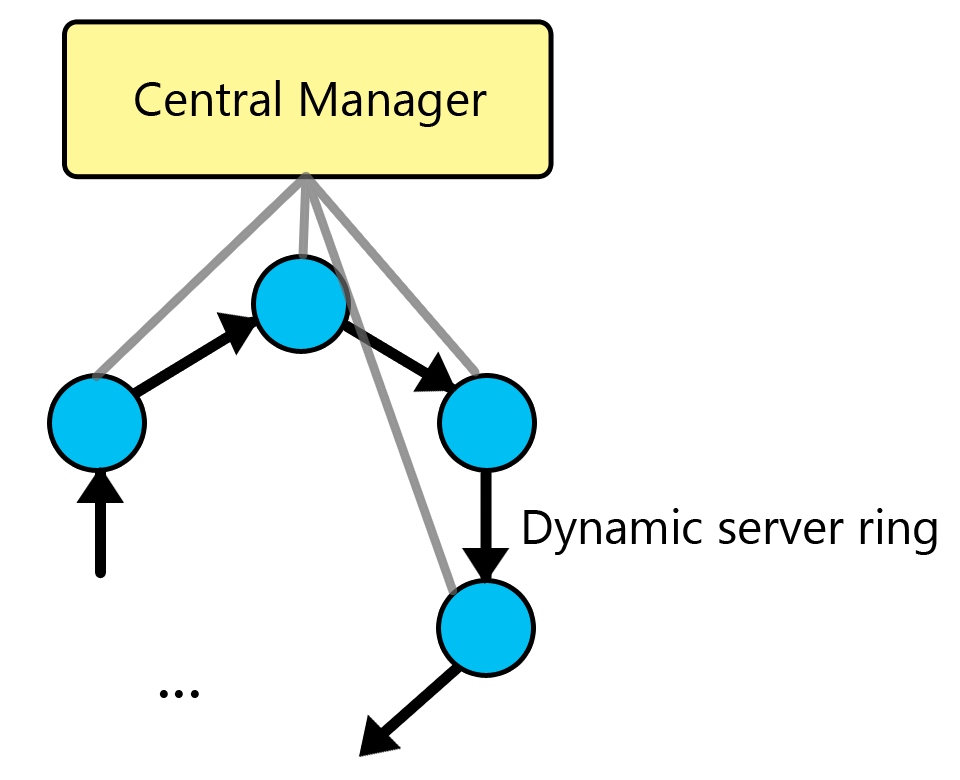
\includegraphics[width=\textwidth]{serverring.png}    
    \end{center}
    \caption{Condor mapped to a server ring}
    \label{fig:serverring}
\end{framed}
\end{wrapfigure}


To get a scalable design in terms of server state synchronization we have utilized a unidirectional ring.
This allows us to handle servers being added and dropped rather easily, as only one existing machine in the ring
will need to be updated for each of these events. An overview of the resulting system can be found in \autoref{fig:serverring}.

The final highlight of our design is that units are stored decentralized.
This means that units use peer-to-peer communication as much as possible for trivial communication (like retrieving the health or type of another unit).
For game critical decisions (like movement or attacking) the server will have to be asked for permission.
The general overview of these event categories and their corresponding assertion levels is shown in \autoref{tab:categories}.

\begin{table}
\begin{tabular}{| l | l | l |}
\hline
\textbf{Category} & \textbf{Communication} & \textbf{Checked by} \\
\hline
\hline
Move related & Server/Client & Full server ring synchronization \\
\hline
Player interaction & Server/Client & Single server validity check \\
\hline
Player information & Peer-to-Peer & No server intervention \\
\hline
\end{tabular}
\caption{Event categories}
\label{tab:categories}
\end{table}

\section{Experimental Results}
\label{sec:results}
\begin{wrapfigure}{l}{0.5\textwidth}
\begin{framed}
    \begin{center}
        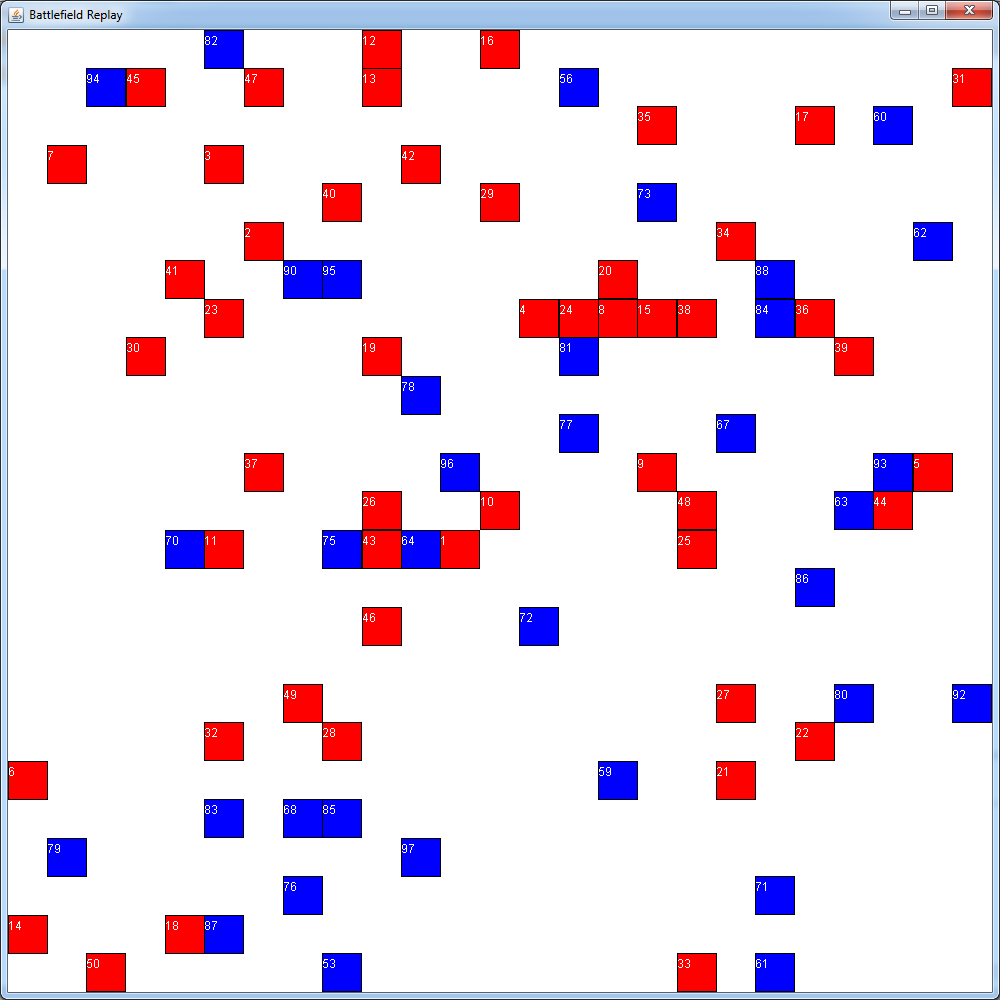
\includegraphics[width=\textwidth]{replay.png}    
    \end{center}
    \caption{Playing a replay}
    \label{fig:replay}
\end{framed}
\end{wrapfigure}

To conduct our experiments we utilized GameTrace logging.
This also allowed us to replay all of the synchronized events using a Replay application we constructed.
It also allowed us to simulate the timings of the events as they happened by using the GameTrace timestamps.
Because the synchronized events include all move related events we can see \textit{spawns}, \textit{moves} and \textit{deaths} of all units in an abitrary GameTrace.
Our replayer only plays single GameTraces, but multiple GameTraces from all Execution Machines could be combined to also reconstruct all \textit{heal} and \textit{damage} events.
A screenshot of a replay being run can be seen in \autoref{fig:replay}.

The initial plan was to run experiments on the DAS4 cluster.
However, due to unexpected problems with the cluster we were forced to do smaller scale testing with two laptops.
The tests we performed are categorized by two deployments: 

\begin{itemize}
\item Single Machine: 1 Physical Machine, 2 Execution Machines
\item Dual Machine: 2 Physical Machines, 2 Execution Machines
\end{itemize}

What we measured was the time until last connect (\autoref{tab:explastconnect}), the  events per second with connection phase(\autoref{tab:expeventswith}),
the events per second without connection phase (\autoref{tab:expeventswithout}) and 
lastly we also measured the performance hit on the system when a server dropped (\autoref{tab:expaggregateloss}).

\begin{table}
\centering
\begin{tabular}{| l | c | c | c |}
\hline
\textbf{Deployment} & \textbf{Clients} & \textbf{Time (ms)}  & \textbf{Time (ms)/Client} \\
\hline
\hline
Single & 10 & 4057 & 405.70\\
\hline
Single & 20 & 11669 &583.45 \\
\hline
Single & 30& 13949 & 464.97\\
\hline
Single & 40& 22604 & 565.10\\
\hline
\hline
Dual & 10 & 2115 &211.50 \\
\hline
Dual & 20 & 5842 &292.10 \\
\hline
Dual & 30 & 14145 &471.50 \\
\hline
Dual & 40 & 12805 &320.13 \\
\hline
\end{tabular}
\caption{Time until last connect}
\label{tab:explastconnect}
\end{table}

\begin{table}
\centering
\begin{tabular}{| l | c | c | c |}
\hline
\textbf{Deployment} & \textbf{Clients} & \textbf{Events/Second}  & \textbf{Events/Second/Client} \\
\hline
\hline
Single & 10 & 47.79& 4.78\\
\hline
Single & 20 &63.35 &3.17 \\
\hline
Single & 30& 69.30& 2.31\\
\hline
Single & 40& 66.91& 1.67\\
\hline
\hline
Dual & 10 & 63.51& 6.35\\
\hline
Dual & 20 & 98.76&4.94 \\
\hline
Dual & 30 & 84.75&2.83 \\
\hline
Dual & 40 &117.51 & 2.94\\
\hline
\end{tabular}
\caption{Events per second with connection phase}
\label{tab:expeventswith}
\end{table}

\begin{table}
\centering
\begin{tabular}{| l | c | c | c |}
\hline
\textbf{Deployment} & \textbf{Clients} & \textbf{Events/Second}  & \textbf{Events/Second/Client} \\
\hline
\hline
Single & 10 & 52.03& 5.20\\
\hline
Single & 20 & 83.59& 4.18\\
\hline
Single & 30&88.76 & 2.96\\
\hline
Single & 40&102.23 & 2.56\\
\hline
\hline
Dual & 10 & 65.72&6.57 \\
\hline
Dual & 20 &111.67 &5.58 \\
\hline
Dual & 30 &  114.03&3.80 \\
\hline
Dual & 40 &147.85 &3.70 \\
\hline
\end{tabular}
\caption{Events per second without connection phase}
\label{tab:expeventswithout}
\end{table}

\begin{table}
\centering
\begin{tabular}{| l | c | c r |}
\hline
\textbf{Deployment} & \textbf{Event} & \textbf{Slowdown (Events/S/Client)} & \\
\hline
\hline
Single & Connection (10 clients) & 0.42  & 8\%\\
\hline
Single & Connection (20 clients) & 1.01  & 24\%\\
\hline
Single & Connection (30 clients) & 0.65  & 21\%\\
\hline
Single & Connection (40 clients) & 0.89  & 35\%\\
\hline
Dual & Connection (10 clients) & 0.22  & 3\%\\
\hline
Dual & Connection (20 clients) & 0.64  & 11\%\\
\hline
Dual & Connection (30 clients) & 0.97  & 26\%\\
\hline
Dual & Connection (40 clients) & 0.76  & 21\%\\
\hline
Dual & Server drop (10 clients) & 3.69  & 56\%\\
\hline
\end{tabular}
\caption{Performance loss per client}
\label{tab:expaggregateloss}
\end{table}

\section{Discussion}
\label{sec:discussion}
The first thing we note is that even though the central manager does not do any of the heavy lifting data-wise, it is a central point of failure.
So even though it scales well, we are not completely happy with it.

Secondly even though the unidirectional ring structure for the execution machines is very scalable and simple to understand,
it comes with a notable performance hit.
To illustrate this: on a single machine utilizing five servers in our distributed structure is about three times as slow as a single server threaded RMI implementation.
Our design should outperform the single server solution due to sheer load though, which is supported by our experiments.

The third thing that we would like to discuss is the load balancing with a dynamic set of servers.
When a server drops the Condor-like load balancing makes sure that the servers receive an equal load of clients.
However, when a new server is added/reconnects it will not balance out the system immediately.
Instead it will simply take in all the new clients and very slowly distribute the load again over time.

\section{Conclusion}
\label{sec:conclusion}
In this project...

\newpage
\section*{Appendix}

\subsection*{A - Time Sheet}
\label{sec:appendix}

\bibliographystyle{plain}
\bibliography{bibliography}

\end{document}
